\section{Introduction}
\label{sec:intro}

\begin{figure}
\centering

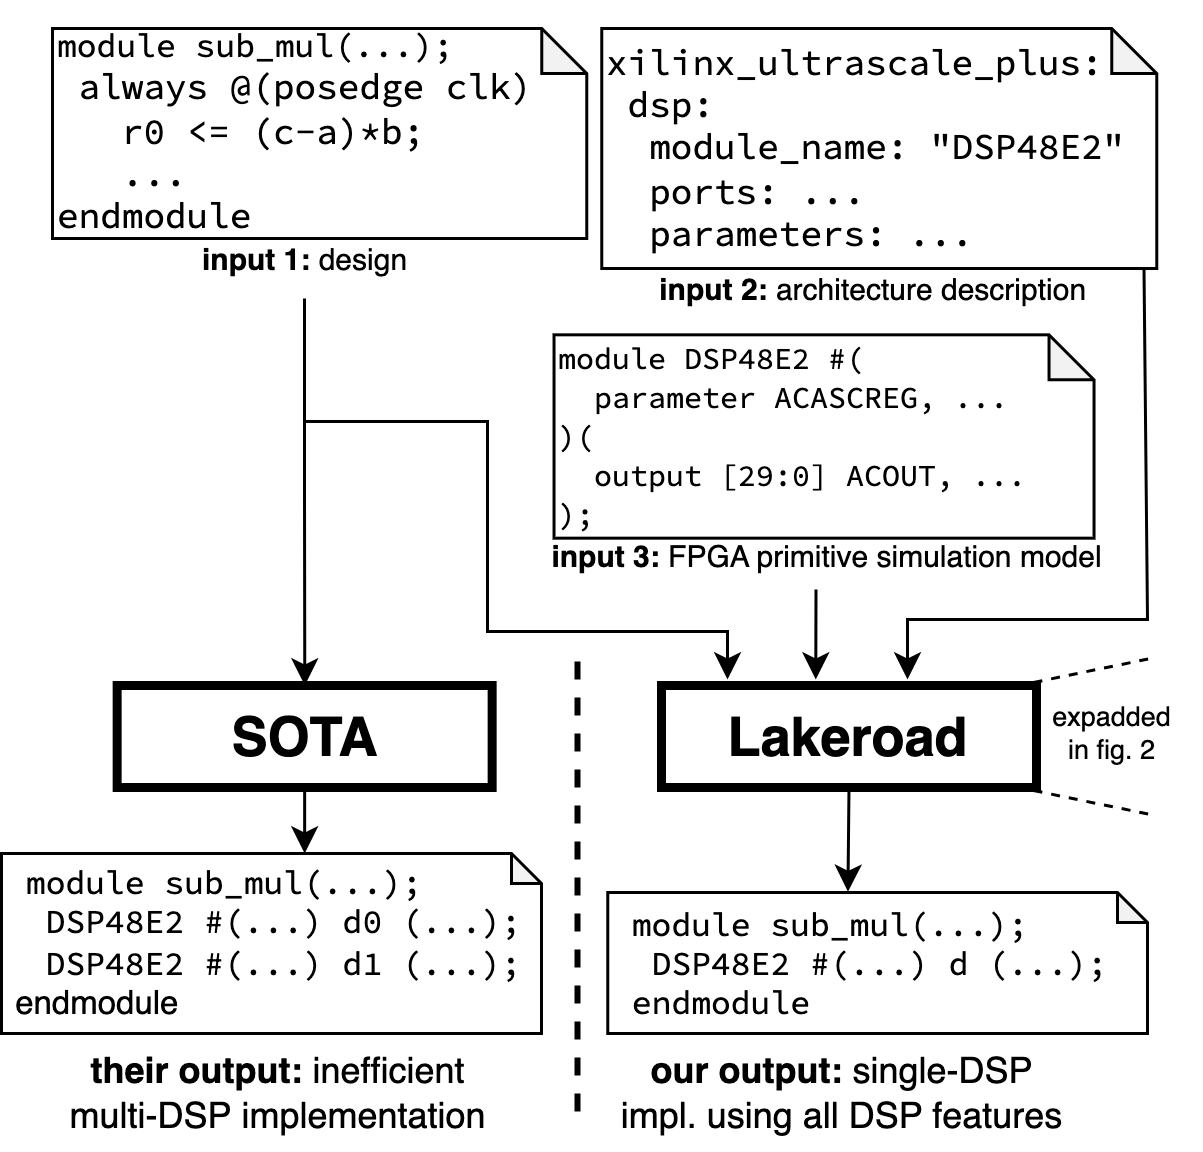
\includegraphics[width=0.91\columnwidth]{assets/lakeroad-firstpage.drawio.png}

% \vspace{3mm}
% \resizebox{0.4\textwidth}{!}{
% \begin{tabular}{cc|c|c}
% Design& \# Stages &  SOTA& \lr \\ \hline
% \texttt{((d+a)*b)|c}& 1 &2 DSP, 18 LUT & 1 DSP  \\
% \texttt{((d+a)*b)\textasciicircum{}c} & 1 & 2 DSP, 18 LUT  & 1 DSP \\
% \texttt{((d-a)*b)|c} & 2 & 2 DSP, 18 LUT & 1 DSP \\
% \texttt{((d-a)*b)\textasciicircum{}c} &  2          & 2 DSP, 18 LUT & 1 DSP \\
% \texttt{((d+a)*b)\&c}& 2 & 2 DSP, 18 LUT & 1 DSP \\
% \end{tabular}}
\vspace{-3mm}
\caption{
% Mapping a simple design to
%   Xilinx UltraScale+ FPGAs with both
%   the state of the art (SOTA)
%   hardware synthesis tool for Xilinx
%   and \lr.
Even given a simple input
  design (input 1),
  the state-of-the-art (SOTA)
  hardware synthesis tool
  for Xilinx FPGAs
  frequently
  fails to efficiently use 
  programmable primitives
  like DSPs.
\lr,
  on the other hand,
  can utilize all features
  of programmable primitives
  given just a short description
  of an FPGA architecture (input 2)
  and the vendor-provided 
  simulation models
  of the primitive (input 3).\tighten
}
\label{fig:firstpage}

\vspace{-5mm}
\end{figure}


Given a high-level hardware design specification
  (e.g., expressed in behavioral Verilog),
  FPGA technology mappers
  search for an equivalent
  low-level implementation
  in terms of the target FPGA's
  primitives.
Recent trends in \textbf{FPGA heterogeneity}---%
  the inclusion of increasingly specialized and diverse primitive elements on FPGAs---%
  have made effective
  technology mapping
  crucial for achieving
  high performance~\cite{vega2021reticle}.
  % possibly relevant cite: zhu2022fpgaheterogeneity

Historically,
  FPGA compute primitives
  consisted primarily of
  generic, homogeneous 
  lookup tables (LUTs) and carry chains.
Automated tools like 
  ABC~\cite{ABC,abc2,brayton2010abc}
  can efficiently map such basic primitives
  by translating \asplos{hardware} designs
  to a library of simple logic gates
  and then packing those gates
  into LUTs.

No comparable
  automatic solution supports
  the wide array of increasingly diverse, highly configurable
  specialized units like digital signal processors (DSPs)
  in modern FPGAs.
For example, Xilinx's DSP48E2
  is a multifunction DSP with over
  100 ports and parameters which
  allow it to
  support a large variety of computations.
  However, this also presents a large search space
  for technology mappers,
  making it challenging
  to correctly configure the primitive
  while also satisfying complex restrictions and dependencies.
% Configuring even a single DSP48E2 is difficult:
%   implementing a given design fragment $D$
%   requires constructing a large configuration
%   that sets each DSP port and parameter
%   to simulate $D$ while also
%   satisfying complex restrictions and dependencies.

Current technology mappers search for such
  configurations via ad hoc, handwritten procedures.
These procedures do not provide strong correctness guarantees;
  recent work highlights the significant number of bugs found across 
  all major hardware synthesis tools~\cite{herklotz2020finding}.
These procedures are difficult to extend;
  \textit{each} new complex primitive requires
  supporting detailed semantics\footnote{
      The Xilinx manual for the DSP48E2 alone
      is over 75 pages long.}
  and adding hundreds of new, special-case
  syntactic pattern matching rules~\cite{wolf2013yosys}.
Finally, these procedures are incomplete;
  they miss many mapping opportunities,
  even across microbenchmarks based on vendor documentation.
\cref{fig:firstpage} (above) shows a
  simple example design consisting of
  \verb-+-, \verb-*-, and \verb-&-,
  which \textit{should} fit on a single DSP48E2,
  but is instead mapped to multiple DSPs and LUTs
  by current state-of-the-art tools.\footnote{
    Licensing restrictions forbid naming the
    specific proprietary tools, but they are familiar,
    standard packages used by many hardware designers.
  }\tighten
  
Our key observation is that
  the configuration space for
  each kind of FPGA primitive
  essentially serves as a small, bespoke
  \textit{programming language}
  that must be used
  to map design fragments
  down to those low-level primitives.
% From this perspective,
%   mapping an HDL design fragment $D$ down to
%   target FPGA-specific primitives
%   reduces to searching for programs
%   (configurations) of the available
%   primitives that are equivalent to $D$.
This paper explores how
  \textit{program synthesis}~\cite{gulwani2017program}
  can be applied to
  simplify the design and implementation of
  FPGA technology mappers while providing
  \textbf{correct},
  \textbf{extensible}, and
  \textbf{more complete}
  support for diverse, highly configurable primitives
  like DSPs.

Program synthesis techniques rely on
  automated theorem provers like
  SAT and SMT solvers~\cite{de2008z3, barbosa22cvc5}
  to automatically generate programs
  satisfying a given specification.
We demonstrate how
  sketch-guided program synthesis~\cite{solar2008program}
  can be adapted
  for FPGA technology mapping:
  given a specification as a
  design fragment $D$ expressed in behavioral HDL,
  we use the Rosette~\cite{torlak2014lightweight} program synthesis framework embedded in the Racket language
  to efficiently search for
  configurations of
  low-level, FPGA-specific primitives,
  i.e., programs in structural HDL
  that implement $D$.\tighten

% We developed two new techniques to enable
%   building correct, extensible, and more-complete
%   FPGA technology mappers
%   via program synthesis:
%   (1) \textbf{semantics extraction from HDL}
%       to provide mostly-automated encoding of the
%       programming language and semantics
%       for each kind of FPGA primitive, and
%   (2) \textbf{architecture-independent sketch templates}
%       to encode generic, high-level implementation strategies
%       that efficiently map design fragments across
%       multiple FPGA architectures.

Sketch-guided program synthesis requires
  encoding the \textit{semantics}
  of the target language:
  in our case,
  a machine-readable,
  mathematical model specifying
  the behavior of each
  FPGA-specific primitive
  being mapped to.
In a typical synthesis tool,
  which generates programs
  for a single target language,
  this is a one-time cost.
However,
  in our setting,
  each new FPGA primitive
  introduces yet another new target language,
  which in turn requires
  extending the tool to encode
  yet another formal semantics.

To support
  \textit{extensible} and \textit{correct}
  technology mapping, we propose
  automating this process with
  \textbf{semantics extraction from HDL}, 
  adapted from past work~\cite{daly2022synthesizing},
  to automatically extract
  complete primitive semantics
  from vendor-published HDL models
  (\cref{fig:firstpage}, ``input 2'').
Traditionally, such models have
   only been used
  for simulation and validation;
  we show that using them for
  target language semantics within a
  program-synthesis-based approach
  yields substantially more
  \textit{complete} FPGA technology mapping.

Sketch-guided program synthesis also
  requires \textit{sketches},
  partially complete programs with ``holes'' to be filled in
  by the solver.
Sketches primarily serve to
  scale synthesis by
  constraining the set of programs that 
  solvers explore when searching for
  one that satisfies
  the given specification,
  i.e., performance at the cost of completeness.
In our setting,
  sketches correspond to
  primitive configurations with
  holes for the port and parameter settings.
The synthesizer will ``fill in the holes''
  as necessary for
  the low-level FPGA-specific primitive to implement
  a given high-level behavioral design fragment.
Unfortunately,
  developing effective sketches
  still requires synthesis expertise~\cite{10.1145/3140587.3062353,vanGeffenJITSynth}.
  Naively, our approach would also
  require new sketches for each new
  FPGA primitive we want to target.


% %Naively, both obtaining
%   %semantics and
%   %writing sketches would
%   %hamper a program synthesis
%   %approach to technology mapping.
% At first glance,
%   obtaining semantics
%   and writing sketches
%   would appear to be difficult
%   manual steps
%   that would impede the use of program synthesis
%   and negating any benefits of automation.
% (Incidentally, current
%   technology mappers also manually
%   specify the semantics
%   via 
%   their unstructured hand-written 
%   patterns and procedures.)
% % Current technology mappers only
% %   reason about primitive semantics
% %   in the unstructured hand-written 
% %   procedures,
% %   and requiring users
% %   to provide sketches
% %   would hamper extensibility, 
% %   as sketches require primitive-specific details
% %   that would negate the automation benefit
% %   of such an approach. 
% However, we apply two key insights
%   to make this approach practical.

 
To address this challenge, 
  we introduce
  \textbf{architecture-independent sketch templates.}
% There are a few common classes 
%   of
%   FPGA primitives
%   present across most architectures:
%   LUTs, carry chains, muxes, and DSPs.
Hardware designs are often implemented
  using similar high-level blueprints
  across most FPGA architectures---%
  sketch templates
  capture these blueprints
  and make them reusable across architectures.
Using sketch templates, we
  greatly reduce the overhead of supporting
  new architectures and
  diverse primitives.
Typically, when adding
  a new primitive, the user
  does not need to write or modify
  any sketch templates.


% However,
%   FPGA primitives across architectures
%   fall into a few common classes, e.g.,
%   LUTs, carry chains, and DSPs, and
%   the way these primitives
%   are used to implement designs
%   is similar across architectures.
% Hence, we introduce abstractions
%   to capture these similarities to build
%   \textbf{architecture-independent
%   sketch templates},
%   reducing the effort required to
%   support a new primitive.



We leveraged these techniques---%
  semantics extraction
  from HDL
  and architecture-independent
  sketch templates---%
  in \lr\footnote{
    \lr is open source and available at
    \textbf{link redacted for anonymity}.
  }, a new FPGA technology mapper
  based on program synthesis.
\lr's prototype implementation automatically
  imports semantics for the LUTs, arithmetic carry chains,
  and DSPs of the Xilinx UltraScale+, Lattice ECP5,
  %Intel MAX,
  and SOFA~\cite{sofa} FPGA architectures. 
The only additional user input to \lr is a short
  architecture description
  %between 20 and 300 source lines 
  %of code,
  which lists the target FPGA's
  primitives.
With the automatically
  extracted primitive semantics
  and the user-provided architecture description,
  we demonstrate that \lr
  is more complete than proprietary tools on a variety
  of microbenchmarks,
  each of which should fit on a single DSP.
In particular,
  we map up to 40$\times$ 
  more designs to 
  DSPs than Yosys, 
  and 1.9--2.7$\times$ 
  more designs than 
  state-of-the-art
  tools for Xilinx and Lattice.\looseness=-1
% We further show the practical applicability
%   of \lr
%   in real-world applications
%   by integrating it into the open-source
%   hardware synthesis tool
%   Yosys~\cite{wolf2013yosys}.

\vspace{1ex}
\noindent
This paper provides 
the following key contributions:
\begin{itemize}
\item A technique for applying
  \textit{semantics extraction from HDL}
  for extensible,
  program synthesis-based
  technology mapping.
\item A design for
  \textit{architecture-independent
  sketch templates.}
\item A language to capture hardware design sketches.
% \item Formal semantics
%   languages for combinational and sequential logic, 
\item A formalization of the \lr
  toolchain, and an argument
  for its correctness as well as
  its completeness modulo sketches.
\item Empirical comparisons of
  \lr and existing hardware synthesis
  tools to evaluate both their
  relative completeness and
  ease of extensibility.


  
% \item The \lr prototype toolchain for
%   practical FPGA technology mapping 
%   via program synthesis.


% \item An evaluation of \lr mapping
%     primitives on Xilinx, Lattice, Intel,
%     and SOFA
%     FPGAs.

\end{itemize}

The rest of this paper is organized as follows.
In \cref{sec:overview},
  we give an overview
  of \lr's design and key features.
In \cref{sec:formalization},
  we formalize \lr and
  demonstrate its correctness.
In \cref{sec:implementation}
  we discuss \lr's implementation.
In \cref{sec:evaluation}
  we evaluate \lr on its
  completeness of mapping,
  extensibility,
  and expressiveness.
  % terms of
  % effort to synthesize technology mappers
  % and the quality of the generated FPGA
  % implementations.
\cref{sec:background-and-related-work}
  discusses related work, and
  \cref{sec:conclusion} concludes.
  


%Modern architectures have traditional 
  %primitives like lookup tables (LUTs) and carry chains,
  %as well as an increasingly diverse array of specialized,
  %highly configurable units like digital signal processors
  %(DSPs).
% In modern FPGAs, types of primitives include
%   both traditional units like
%     lookup tables (LUTs) and  carry chains,
%   as well as an increasingly diverse array of
%     specialized, highly configurable units like
%     digital signal processors (DSPs). 
% For these traditional units, automated tools like 
%     ABC~\cite{ABC,abc2,brayton2010abc}
%     can achieve high-quality mapping results
%     in the context of
%     homogeneous
%     FPGAs (consisting only of
%     LUTs)
%     by efficiently mapping designs
%     to a library of simple logic gates
%     and then packing those gates
%     into LUTs.
% Today's specialized primitives are highly complex
%   and sophisticated, requiring significant knowledge
%   of their behavior to use effectively.


% \hline
% 
% % What is technology mapping
% Technology mapping
%   is one step
%   in the process of mapping
%   a hardware design
%   onto an FPGA.
% During technology mapping,
%   FPGA synthesis tools
%   determine how to implement
%   the high-level description
%   of the design
%   using an FPGA platform's
%   specific primitives.
% To compile designs effectively,
%   it is critical that technology mappers
%   utilize all available types of primitives
%   on an architecture, e.g.,
%   lookup tables (LUTs),
%   carry chains, and
%   digital signal processors (DSPs).
%  
% % Technology mapping is difficult to implement.
% Technology mapping is difficult to implement.
% % What can we say in the general case? We don't know how it's implemented in Vivado, Diamond.
% Generally, technology mappers
%   apply a combination of
%   low-level,
%   automated search
%   and
%   high-level, hand-written
%   pattern matching
%   to explore potential mappings
%   of designs to primitives.
% For example,
%   the Yosys synthesis suite~\cite{wolf2013yosys}
%   utilizes the logic synthesis tool ABC~\cite{abc}
%   automatically map hardware designs
%   to simple gates with concrete semantics,
%   such as \texttt{AND}, \texttt{OR},
%   and \texttt{NOT},
% % Is conversion to LUTs special-cased?
% % See https://people.eecs.berkeley.edu/~alanmi/abc/
%   and then packs those gates
%   into look-up tables (LUTs).
% Though this process is automatic,
%   it is limited to simple primitives.
% 
% % Increasing heterogeneity is good, dsps are good
% To increase performance
%   and decrease power,
%   FPGAs are becoming increasingly heterogeneous.
% While originally FPGAs were homogeneous arrays
%   of LUTs,
%   FPGAs now include primitives
%   specialized for common task,
%   such as arithmetic carry chains.
% Beyond specialized combinational logic,
%   increasingly FPGAs include
%   \textit{digital signal processors}
%   (DSPs):
%   complex programmable primitives with a
%   wide range of potential behavior.
% When utilized correctly,
%   DSPs significantly boost the performance
%   of compiled hardware designs.
% 
% % but Increasing heterogeneity makes techmapping harder
% While heterogeneity
%   gives hardware designers access
%   to specialized primitives,
%   it also increases the difficulty
%   of technology mapping.
% Each new primitive
%   must be supported
%   in the current technology mapping solution.
% This requires
%   
% Cite RapidWright~\cite{lavin2018rapidwright}
% 
% % This needs to be broken into multiple paragraphs:
% % - What is sketch-guided program synthesis
% % - Sketch-guided program synthesis is usually used in constrained cases. Previously, FPGA technology mapping was not constrained, i.e. one big search with ABC. however, new compilers break the problem down into instructions. Program synthesis now becomes feasible.
% % - Uses sketches capture useful, general patterns and constrain search (in contrast to ABC and other techniques?)
% % - But requires semantics to work
% 
% % Semantics are already available in vendor provided models! We extract them, even for large, 1000+ line Verilog models of DSPs
% 
% 
% % Our tool lakeroad encapsulates all of these techniques
% 
% % our results
% 
% %
% 
% 
% \hline
% 
% %Powerful FPGA synthesis tools
% %  are critical
% %  in the hardware design process.
% FPGA synthesis tools
%   enable hardware designers
%   to be productive.
% Rather than needing to write
%   low-level, FPGA-specific
%   HDL 
%   (hardware description language)
%   code,
%   a hardware designer is instead
%   able to write
%   high-level,
%   architecture-independent
%   HDL,
%   which the synthesis tool
%   will compile into a low-level implementation
%   which efficiently uses
%   the FPGA's resources.
% 
% Synthesis tools
%   are massive engineering projects.
% Many of the best tools---%
%   such as Xilinx's Vivado~\cite{vivado}
%   and Lattice's Diamond~\cref{diamond}---%
%   are developed by teams of many engineers
%   at large FPGA companies.
% Yosys~\cite{wolf2013yosys},
%   an open-source FPGA synthesis tool,
%   has over 11,000 commits
%   representing contributions 
%   from nearly 200 people.
% 
% One of the biggest hurdles
%   in building synthesis tools
%   is in supporting new FPGA architectures.
% Not only does this require experties
%   in the synthesis tool itself,
%   but it also requires knowledge
%   of the underlying FPGA architecture.
% Each architecture can add 
% 
%   which can be a high bar 
%   especially
%   for developers
%   of open-source FPGA synthesis tools.
%   
% To reduce some of the implementation burden,
%   FPGA synthesis tools rely on
%   \textit{technology mapping}
%   tools 
%   %such as ABC
%   to automatically, 
%   flexibly map designs
%   to 
%   FPGA-specific primitives.
% Traditionally, however,
%   technology mapping has been limited to small, 
%   fixed-function primitives, 
%   and does not support large programmable units like DSPs.
% %  
% In this paper,
%   we present a new method of technology mapping
%   which can utilize
%   all primitives available on an FPGA architecture---%
%   not just LUTs, but carries and even DSPs.
% Our method utilizes
%   \textit{sketch-guided program synthesis}
%   and \textit{semantics extraction from HDL}
%   to determine the behavior
%   of FPGA primitives automatically.
% Our method requires little user input,
%   and integrates into and enhances 
%   existing FPGA synthesis approaches.
% 
% 
% \hl{make it clear up front that we're doing tech mapping, not placement}
% 
% \hl{we need to put the comparison-on-carry trick somewhere}
% 
% Field-programmable gate arrays (FPGAs)
%   are a popular platform
%   for developing custom hardware
%   due to their
%   performance,
%   affordability,
%   and reprogrammability.
%  FPGA technology
%   continues to advance, with
%   FPGAs becoming increasingly
%   complex.
% Whereas early FPGAs
%   were homogeneous arrays of 
%   \textit{lookup tables} (LUTs)---%
%   configurable memory devices that can be programmed
%   to implement bitvector functions ---%
%   modern FPGAs are 
%   heterogeneous,
%   containing
%   increasingly complex
%   specialized units
%   such as dedicated
%   carry chains
%   and digital signal processors (DSPs).
%   
% Though FPGA hardware has advanced,
%   their software toolchains have not, and legacy toolchains
%   struggle to support modern heterogeneous
%   FPGAs~\cite{lavin2018rapidwright}.
% %
% Legacy toolchains use \textit{hardware synthesis}---a complex process
% that attempts to infer high-level structure (e.g., a pipelined multiplier)
% from a low-level representation (e.g., an and-inverter graph).
% %
% Hardware synthesis is at the root of legacy toolchains'
% struggle or outright inability to utilize
% specialized units of modern FPGAs.
% 
% Legacy toolchains struggle to utilize specialized units on FPGAs
%   because their approach to \textit{hardware synthesis}
%   attempts to translate input programs to FPGA designs in
%   ``one big step''.
% Such tools attempt to automatically infer high-level structure---%
%   such as an entire pipelined multiplier---%
%   from a low-level representation---%
%   such as an and--inverter graph---%
%   via heuristics which have not scaled well
%   as FPGA heterogeneity increases.
% 
% % At the root of 
% %  legacy toolchains' difficulty
% %  in utilizing specialized units
% %  is
% %  the tools' use of
% %  \textit{hardware synthesis,}
% %  a complex process which attempts to infer
% %  high-level structure---%
% %  such as an entire pipelined multiplier---%
% %  from a low-level representation---%
% %  such as an and--inverter graph---%
% %  via a brittle process of pattern matching.
% 
% 
% In contrast,
%   software compilers typically generate
%   their output by progressively lowering
%   source-level code down to machine-level code via
%   a sequence of semantics-preserving transformations.
% Several recent hardware compilers designed to target FPGAs
%   have also adopted such a progressive lowering strategy~\cite{
%     vega2021reticle, nigam2021compiler, circt}.
% As in traditional compilers,
%   the lowest-level IR in these compilers must be transformed into
%   output code by an target-specific backend,
%   e.g., to target a Xilinx UltraScale+ FPGA,
%   such compilers would need a pass that translates
%   the lowest-level hardware-agnostic intermediate representation (IR)
%   into UltraScale+ specific HDL code.
% 
% 
% Compared to traditional hardware synthesis,
%   progressive compilation facilitates
%   mapping high-level expressions down to
%   complex FPGA components by preserving
%   high-level structure until late in the
%   compilation pipeline.
% In contrast, traditional synthesis
%   translates entire designs into
%   graphs of gates, thus losing high-level information.
%   (TODO PATCH UP THIS PARA)
% 
% 
% % Recently,~\citet{vega2021reticle} introduced Reticle,
% %   a compiler for FPGA designs,
% %   which replaces hardware synthesis with
% %   \textit{progressive lowering compilation.}
% % In this style of compilation,
% %   FPGA hardware designs are lowered gradually
% %   from high-level (e.g., Verilog) to low-level (e.g., LUT and DSP configurations),
% %   inferring hardware primitives along the way.
% % This allows high-level expressions
% %   with complex low-level implementations
% %   (such as multiplies)
% %   to be discovered and mapped to specialized hardware
% %   more easily.
% 
% % Software compilers typically generate
% %   their output by progressively lowering
% %   source-level code down to machine-level code via
% %   a sequence of semantics-preserving transformations.
% % Several recent hardware compilers designed to target FPGAs
% %   have also adopted such a progressive lowering strategy~\cite{
% %     vega2021reticle, nigam2021compiler, circt}.
% % As in traditional compilers,
% %   the lowest-level IR must be transformed into
% %   output code by an target-specific backend,
% %   e.g., to target a Xilinx UltraScale+ FPGA,
% %   such compilers would need a pass that translates
% %   the lowest-level hardware-agnostic intermediate representation (IR)
% %   into an UltraScale+ specific HDL code.
% 
% 
% % Progressive lowering compilers
% %   transform programs to a target lowest-level representation
% %   often called the instruction set architecture or ISA.
% % Building a progressive lowering compiler
% %   requires a well-defined 
% %   lowest level of representation,
% %   often called the
% %   \textit{instruction set architecture (ISA)},
% %   to which a design should be lowered.
% % Several recent compilers designed to target FPGAs
% %   adopt a progressive lowering strategy.
% % As in traditional compilers,
% %   the lowest-level IR must be transformed into
% %   output code by an target-specific backend.
% 
% % This low-level IR
% %   must be then compiled to FPGA-specific code
% %   for each FPGA backend the compiler targets.
% % This has problems x y z...
%   
%   \hl{Ben: the following disembodied hunk seems left over from an edit}
%   several recent compilers for FPGAs
%   released in the past five years 
%   are designed
%   
%   include
%   an ISA at the core of their design.
% For example, the ISAs of
%   Reticle~\cite{vega2021reticle},
%   Calyx~\cite{nigam2021compiler},
%   and the MLIR CIRCT project~\cite{circt}
%   are composed of
%   logic instructions such as \texttt{and} and \texttt{or},
%   arithmetic instructions such as \texttt{add} and \texttt{sub},
%   and other instructions such as
%   \texttt{mux} and shifts.
%  
% Modern FPGA compilers use one
%   of two approaches to implement
%   their ISAs, and each of these
%   approaches have their own
%   limitations.
% The first method,
%   used by Calyx and MLIR CIRCT,
%   generates high-level
%   \textit{behavioral Verilog},
%   and then relies on traditional
%   hardware synthesis
%   for compilation.
% This approach loses
%   many of the benefits
%   we gain
%   from switching to
%   progressive lowering-based compilation.
%   
% The second method,
%   used by Reticle,
%   implements
%   the ISA for each backend manually
%   by providing a low-level
%   \textit{structural Verilog}
%   implementation
%   of each instruction
%   in terms of the specific FPGA's
%   primitives (e.g.~LUTs, DSPs, and carry chains).
% This method retains the
%   benefits of progressive
%   lowering compilation lost
%   by the first method, but
%   currently requires a hand-written
%   ISA which does not scale:
%   as the number of ISA instructions 
%   and the number of FPGA backends grow
%   (e.g., as we consider fusions of instructions,
%   or instructions specialized with constant values)
%   it becomes infeasible to implement
%   each instruction
%   for each backend.
% Implementing low-level ISAs by hand
%   can also lead to bugs,
%   especially on FPGA architectures
%   with complicated hardware primitives
%   such as DSPs.
% Additionally,
%   implementing ISAs by hand
%   requires expertise,
%   and as FPGAs become more heterogeneous,
%   implementers may miss
%   crucial opportunities
%   to utilize all available specialized units---%
%   for example, utilizing arithmetic carry chains
%   to implement non-arithmetic functions
%   such as comparisons~\cite{todo} % there are two citations for this.
% \hl{This point might motivate us needing
% to implement more than one version of an ISA, and this
% can be used to argue that implementin by hand is
% not scalable. Is there a way to put this before
% that point?}
% Finally,
%   this approach locks in a single instruction implementation
%   for the entire compiler,
%   but different optimization goals
%   (e.g.~design latency vs design area) might require different implementations.
%   
% 
% Implementing FPGA ISAs is an ideal use case
%   for sketch-guided program synthesis---%
%   a technique that
%   uses an SMT solver
%   to fill in holes
%   in \textit{program sketches}.
% Generally, sketch-guided program synthesis
%   performs best
%   when the domain 
%   is finite and loop-free,
%   and the program being synthesized
%   is small.
% FPGA ISA instruction implementations
%   fit this description.
% Their domain is the domain of bitvectors,
%   which SMT solvers reason about
%   efficiently.
% Furthermore, an instruction implementation
%   will be small and simple,
%   generally composing just a few FPGA primitives
%   to implement the requested instruction.
% 
% \hl{Ben: I'm gonna take another stab at these paragraphs, but I'm leaving
% the original in}
% While the domain of implementing FPGA ISAs
%   is an ideal application for sketch-guided
%   program synthesis, program synthesis
%   requires the user to provide the
%   semantics of the target
%   language---in our case, the semantics
%   of the target FPGA's primitives.
% Generally users of program synthesis
%   have to provide these semantics by
%   hand-writing an interpreter for their
%   domain.
% This would be too much work to ask of end users,
%    and we avoid this by automatically generating
%    interpreters for FPGA primitives from
%    vendor-provided Verilog simulation models
%    of the primitives.
% 
% \hl{original version}
% However, program synthesis
%   requires the user to provide
%   the semantics of the target language---%
%   in our case, the language of hardware design.
% Generally, users of program synthesis
%   provide these semantics
%   by writing an interpreter
%   for their domain.
% However, FPGA vendors release
%   Verilog simulation models
%   of their FPGAs' primitives;
%   these simulation models provide
%   exact semantics for the primitives.
% We need only to make these semantics
%   available to the program synthesis tool
%   to be able to do synthesis for a given FPGA.
% \hl{end original}
% 
% 
% In this work
%   we use sketch-guided program synthesis
%   to synthesize ISA implementations
%   for different FPGA backends.
% To represent sketches,
%   we present 
%   a domain-specific language,
%   \lrir,
%   with two levels of abstraction:
%   an architecture-independent level
%   of \textit{sketch templates,}
%   which capture abstractions
%   common among many FPGAs,
%   and an architecture-specific level.
% Furthermore,
%   we demonstrate how to automatically extract
%   the
%   semantics
%   of architecture-specific FPGA primitives
%   necessary for program synthesis
%   directly from the Verilog models
%   released by hardware vendors.
% \lr is fast \hl{insert some result} and
%   its outputs are correct by construction:
%   we provide a formalization of \lr
%   and argue for its correctness.
% \lr also allows users to explore
%   tradeoffs between instruction implementations
%   by discovering multiple implementations
%   for a given instruction.
% Lastly, \lr
%   can enable support for new architectures
%   with little effort from the end user.
%   \hl{should emphasize this way more}
%   
%   
% % For framing the contributions
% % https://www.cs.tufts.edu/~nr/pubs/tiler.pdf
% %https://theory.stanford.edu/~aiken/publications/papers/pldi16a.pdf
% %https://pp.ipd.kit.edu/uploads/publikationen/buchwald18cgo.pdf
% 
%   
% %Through our work,
%   %we also seek to demonstrate our thesis
%   %that compilation
%   %should originate
%   %from the semantics of hardware---%
%   %semantics which are formally captured
%   %in many forms today,
%   %such as in Verilog implementations of the design.
% %
% %Furthermore, beyond our tool,
%   %we propose a fundamental shift
%   %in how the field thinks about
%   %hardware design.
% %Namely, we demonstrate that
%   %\textit{formal hardware models}
%   %of a hardware platform's primitives
%   %are useful for more than
%   %validation or verification
%   %of human-made designs---%
%   %they can in fact be used
%   %to build automated reasoning tools
%   %which design hardware automatically.
% %In this paper,
%   %we present our first demonstration of this idea
%   %in the limited scope of FPGAs,
%   %as FPGAs are well-established
%   %and FPGA vendors generally release
%   %Verilog models of their architectures.
% %However, 
%   %we believe this idea extends to
%   %\textit{any} hardware platform
%   %whose primitive blocks
%   %are modeled formally.
% 
% Concretely, our contributions are:
% \begin{itemize}
% \item The conceptual insight that sketch-based program synthesis
%   can be used to implement
%   FPGA ISAs.
%   
% \item A two-level domain-specific language, \lr.
% 
% \item Sketches implemented in \lr
%   which capture design patterns
%   common across multiple FPGA platforms.
% These sketches are sufficient for synthesizing entire ISA
%   implementations
%   on new FPGA architectures.
%   
% \item A framework which allows users
%   to easily generate new
%   architecture-independent
%   or
%   architecture-specific sketches.
% 
% \item A method for extracting hardware semantics directly from
%   Verilog simulation files
%   provided by FPGA vendors,
%   and an open-source implementation
%   of the method.
%   
% \item An abstraction which allows
%   the semantics of stateful designs
%   to be represented in SMTLib-like syntax.
% 
% 
% \item An evaluation of Lakeroad, including
%   \begin{enumerate}
%       \item A per instruction quantiatative analysis of our ISA for Xilinx Ultrascale+, Lattice ECP5, and SOFA\cite{sofa}.
%       \item A demonstration of integrating \lr-generated instructions into multiple external frameworks (Calyx and MLIR CIRCT).
%       \item A case study, demonstrating the ability of \lr to generate implementations for 
%         SOFA, an FPGA architecture
%         otherwise unsupported
%         by most hardware compilers.
%   \end{enumerate}
%   
% \item A functional, open-source, and documented implementation of the tool, available on GitHub.
% \end{itemize}
% %
% %\hl{A key part of the story: FPGAs are going to keep getting more diverse. See recent Google work (FPGA22, HPCA? talk to luis, see slack) about Google's work on new FPGAs}
% 
% % \hl{end intro from Generals}
% 
% % \hl{luis begin}
% % 
% % There is an increasing number of domain-specific languages and compiler
% % infrastructure built for the purpose of describing hardware more efficiently,
% % including calyx, llhd, circt, etc. (add more information about these languages here)
% % 
% % All of these languages use behavioral Verilog as a low-level IR, which in turn can be used for both programming FPGAs and designing ASICs.
% % 
% % Nevertheless, behavioral Verilog is known to be inefficient for programming modern
% % FPGAs, requiring programmers to write brittle low-level and target-dependent implementations to unleash the maximum potential of these architectures.
% % Interestingly, some recent work (reticle) has shown a new approach to program
% % modern FPGAs using software compiler techniques, based on instruction selection,
% % leading to faster compilation times at expense of resource utilization in some
% % cases.
% % 
% % Sadly, one challenge of this work is that the target description or rewrite rules,
% % used by the instruction selector, are written by hand which it is error-prone and
% % limits the number of architectures that can be supported over time. The main goal
% % of an intermediate representation is to support as many targets as possible.
% % 
% % We propose a technique (or case study) on how to use program synthesis plus
% % something else to automatically learn/derive/search these implementation without
% % human intervention. We show that this approach cannot only be leverage by reticle-like
% % languages, but also other languages like calyx or dialects in circt. These languages
% % now can be lowered directly to FPGA primitives without relying on traditional
% % hardware synthesis, and target at the same time all these new FPGA architectures that
% % are going to be available (we can lean hard on the fact that people are building
% % their own FPGAs now because of OpenFPGA frameworks and this is not a story
% % of Amd and Intel anymore). The more the targets the better it is to have a technique
% % that automatically figure all this out.
% % \hl{say "dialect", people like that}
% % 
% % Maybe we can say also that another benefit of this work is that equivalence
% % checking is no longer required because the process of translating an intermediate
% % language to FPGA primitves is now sound, due to program synthesis, compared
% % to traditional hardware synthesis. I am not so sure about this but we can
% % see how the stoke paper was written.
% % 
% % \hl{luis end}
% 
% 
% \hl{The rest of this paper is organized
%   as follows...}